\documentclass[a4paper, 10pt, twocolumn]{article}
\usepackage{graphicx} % Required for inserting images
\usepackage[utf8x]{inputenc}
\usepackage[english,russian]{babel}
\usepackage{cmap}
\usepackage[left=1cm,right=1cm,
    top=1cm,bottom=1cm]{geometry}
\usepackage{paracol}
\usepackage{multicol}
\usepackage{amsmath}
\usepackage{lipsum}
\usepackage{vwcol} 
\usepackage{float}
\usepackage{cancel}
\usepackage[normalem]{ulem}
% Установка размера формул
\DeclareMathSizes{10}{10}{10}{10}   % Для основного текста размером 10pt

\title{Вопрос по выбору \\ Циклоидный маятник}
\author{Матвей Галицын \\ Б01-411}
\date{November 25, 2024}

\setlength{\columnseprule}{0.1pt}
\setlength{\columnsep}{3em}

\begin{document}
\maketitle
\newpage{}
\section*{Что же такое циклоида?}
    Циклоида может быть описана траекторией точки, зафиксированной на окружности, которая катится по 
    прямой без проскальзывания с постоянной скоростью.

    Система уравнений, задающих такую траекторию, получается достаточно просто. Это по-сути суперпозиция 
    вращательного движения вокруг центра масс колеса и поступательного движения 
    центра колеса. Притом если т. O покоится, то  $$[\vec{\omega} \times \vec{R}] = \vec{v} \eqno{(1)}$$

    Провернем колесо на небольшой угол. Точка как поднялась, так и сдвинулась по горизонтали. Тогда система, 
    описывающая такую траекторию, описывается параметрическими уравнениями. Начальное положение точки берм в 
    точке соприкосновения колеса и пов-ти. Длина дуги $R\cdot\phi$ равна смещению центра по OX, это следует 
    из (1). Смещение по OX = смещение центра + смещение, связанное с вращением. 
    \begin{equation*}
        \begin{cases}
            x(\phi) &= R\cdot\phi - Rsin(\phi)\\
            y(\phi) &= R (1 - cos(\phi))
        \end{cases}
        \eqno{(2)}
    \end{equation*}

    Маленькая длина пути, пройденная точкой на окружности можно найти следующим образом: 
    $$dS = \sqrt{\left(\frac{dx}{d\phi}\right)^2 + \left(\frac{dy}{d\phi}\right)^2} \cdot d\phi = 
    \sqrt{x_\phi^\prime + y_\phi^\prime} \cdot d\phi\ \eqno{(3)}$$

    При этом из системы (2) имеем: $x_\phi^\prime = R(1-cos(\phi))$, а $y_\phi^\prime = sin(\phi)$. Подставляем 
    теперь это в (3) и получаем малое приращение длины дуги кривой: \\
    $dL = R\sqrt{2-2cos(\phi)} \cdot d\phi = \sqrt{2}R\sqrt{1-cos(\phi)} \cdot d\phi= \sqrt{2}R\sqrt{2{sin}^2
        (\frac{\phi}{2})} \cdot d\phi=2R \cdot sin\left(\frac{\phi}{2}\right) d\phi$ \\

    Тогда полная длина дуги циклоиды: 
    $$L = 2R\int_{\phi_{0}}^{\phi} sin\left(\frac{\phi}{2}\right) d\phi = -4R \cdot cos\left(
        \frac{\phi}{2}\right)\Bigg|_{\phi_0}^{\phi} $$
    $$ L = 4R\cdot\left(cos\left(\frac{\phi_0}{2}\right) - cos\left(\frac{\phi}{2}\right)\right) \eqno{(4)} $$
\section*{Как получается циклоидный маятник?}
    Берется окружность, плотно прижатая к поверхности, и проводится траектория точки, которая изначально
    находилась снизу. Делается один полный оборот. \\
    \begin{figure}[H]
        \centering
        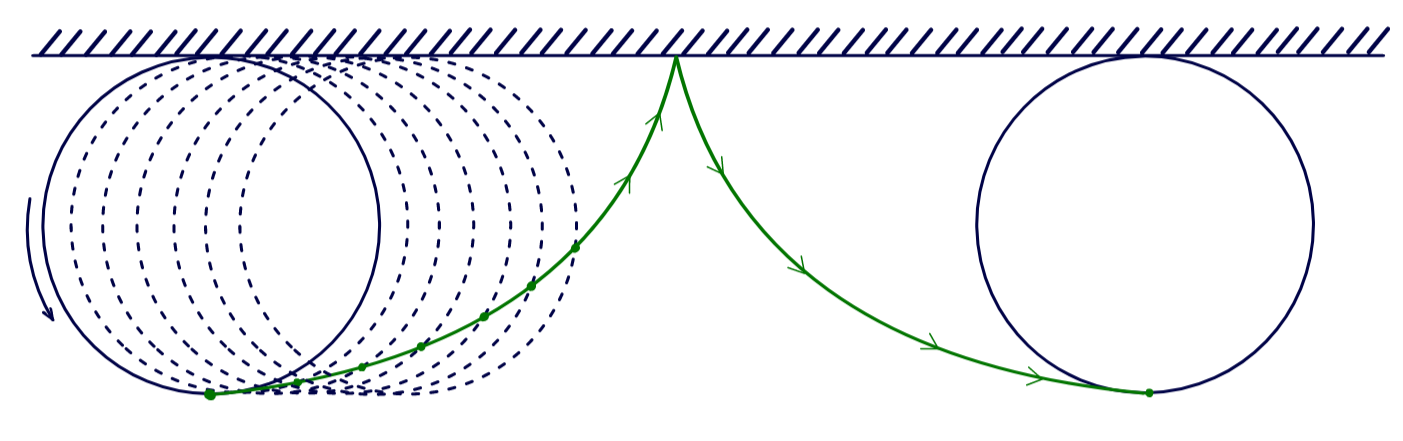
\includegraphics[width=1\linewidth]{traectory1.png}
        \caption{Первая часть построения циклоидного маятника}
    \end{figure}
    Далее берется абсолютно такая же окружность и аналогичным образом проводится траектория точки, которая
    изначально была сверху у окружности.
    \begin{figure}[H]
        \centering
        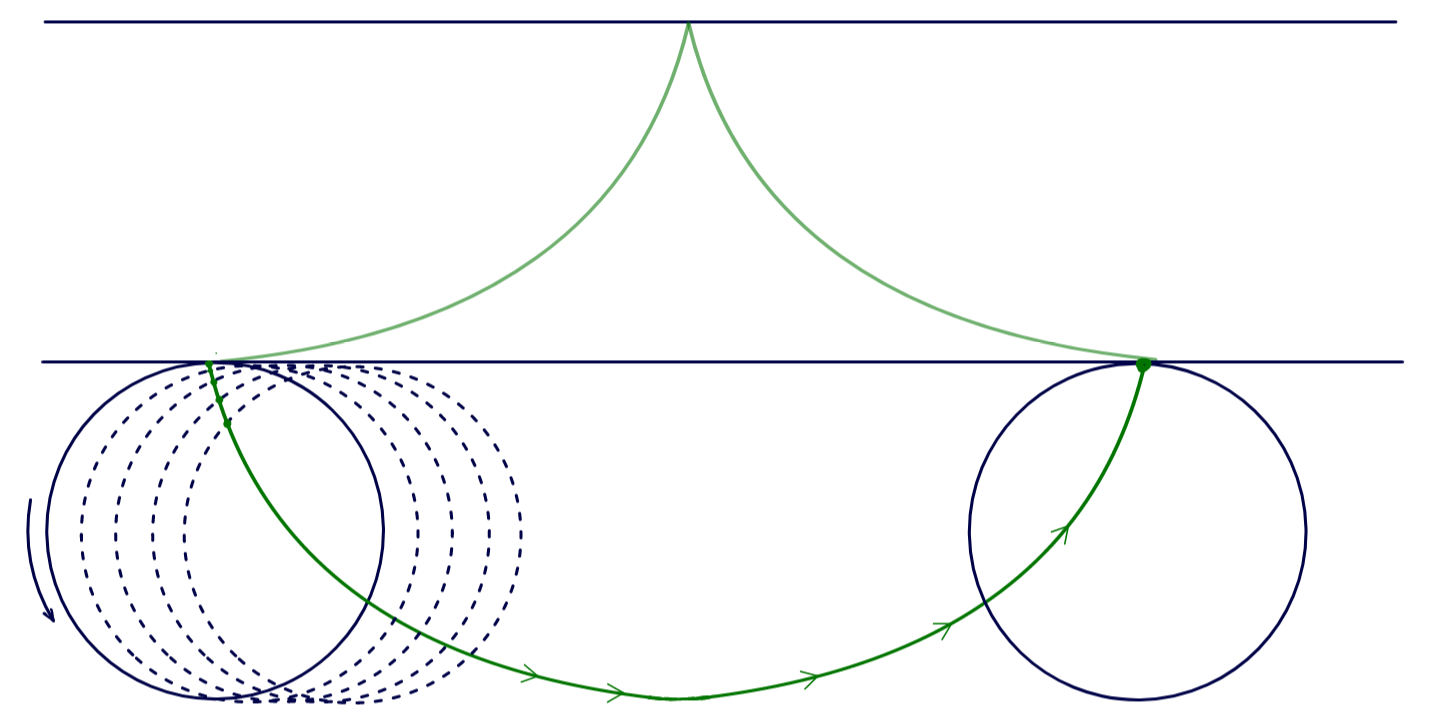
\includegraphics[width=1\linewidth]{traectory2.png}
        \caption{Вторая часть построения циклоидного маятника}
    \end{figure}
    Из формулы (4) видно, что при повороте колеса на угол  $\pi$, длина дуги, описанной произвольной
     точкой на дуге колеса, будет равна 4R. То есть половина длины дуги циклоиды равна четырем радиусам
     самого колеса. И тогда понятно, что если взять точечное тело на нитке длиной 4R, то оно будет 
     колебаться по нашей замкнутой фигуре следующим образом:
     \begin{figure}[H]
        \centering
        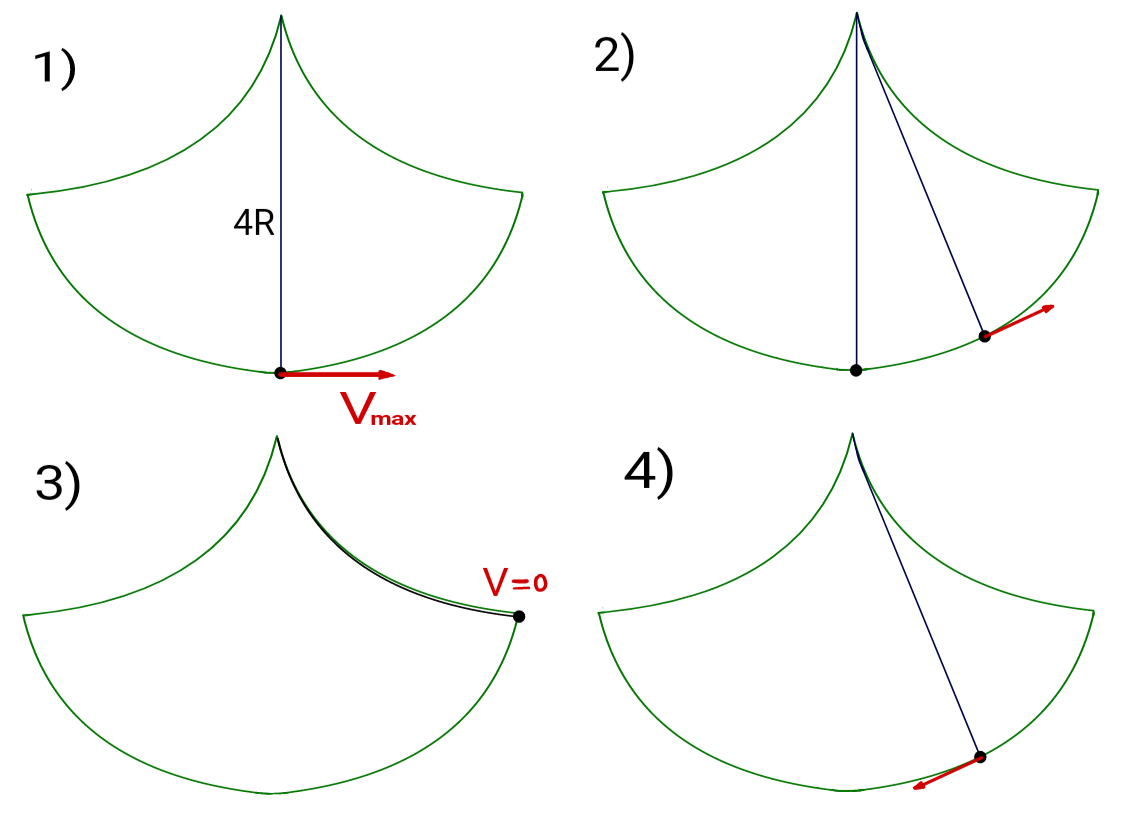
\includegraphics[width=1\linewidth]{kolebania1.png}
    \end{figure}
    \begin{figure}[H]
        \centering
        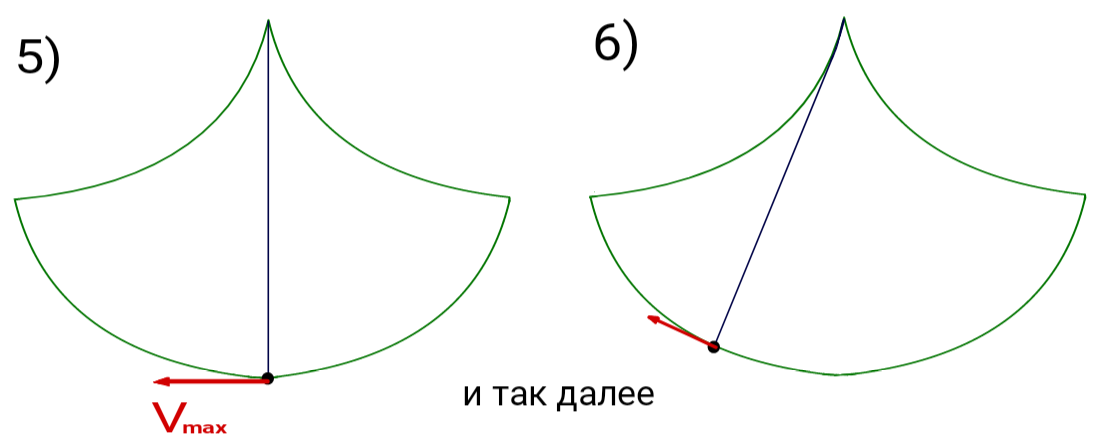
\includegraphics[width=1\linewidth]{kolebania2.png}
        \caption{Иллюстрация колебаний маятника}
    \end{figure}
    Берется две одинаковые окружности, плотно прижатые друг друг. Такую систему двигают с постоянной скоростью
     V. При этом проскальзывания между нижним кольцом и поверхностью также нет. Очевидно отгда, что скорости точек соприкоснования колес в 
    ЛСО одинаковы и равны $2v$ (нет проскальзывания).
\section*{Период колебаний}
    Период колебаний достаточно легко найти из \textbf{закона сохранения энергии}. \
    Запишем: $$ \text{K} + \text{П} = const $$
             $$ \frac{1}{2}mV^2 + mg(y - y_0) = const $$
    C учетом $y(\phi)$ из (2), $V = \frac{dS}{dt}$ и формулы (4) получается система:
    \begin{equation*}
        \begin{cases}
            \frac{1}{2}mV^2 + mg(y - y_0) = const \\
            V = \frac{dS}{dt} \\
            y(\phi) = -R (1 - cos(\phi)) \\
            S(\phi) = 4R\cdot\left(cos\left(\frac{\phi_0}{2}\right) - cos\left(\frac{\phi}{2}\right)\right)
        \end{cases}
    \end{equation*}
    Решим данную систему: \\
    Продифференцируем $S(\phi)$:
    $$ S^\prime = -2R \sin\left(\frac{\phi}{2}\right) \cdot \phi^\prime $$
    Возьмем const = 0, тогда получим:
    $$ \frac{1}{2}mV^2 + mg(y - y_0) = 0 $$
    $$ \frac{1}{2}mV^2 = mg(y_0 - y) $$
    $$ 2R^2sin^2(\frac{\phi}{2}){\phi^\prime}^2 = g(y_0 - y) = gR(cos(\phi_0) - cos(\phi)) $$
    $$ 2R \cdot \frac{1 - cos(\phi)}{2} \cdot {\phi^\prime}^2 = g(cos(\phi_0) - cos(\phi)) $$
    $$\downarrow$$
    $$ \frac{d\phi}{dt} = \sqrt{\frac{g}{R} \cdot \frac{cos(\phi_0) - cos(\phi)}{1 - cos(\phi)}} \eqno{(5)}$$
    Т.к. в начале $\phi_0 = 0$, то $cos(\phi_0) = 1$, получим:
    $$ \frac{d\phi}{dt} = \sqrt{\frac{g}{R} \cdot \frac{1 - cos(\phi)}{1 - cos(\phi)}} = \sqrt{\frac{g}{R}} $$
    \begin{equation*}
        \frac{d\phi}{dt} = \left\{
                \begin{array}{ll}
                    \sqrt{\frac{g}{R}}, \text{ при движение \textbf{справа налево}} \\
                    -\sqrt{\frac{g}{R}}, \text{ при движение \textbf{слева направо}}
                \end{array}
            \right.
    \end{equation*}
    Уже понятно, что это не обычный математический маятник. Интересный факт, что угловая скорость
    маятника не зависит от времени, как это происходит в обычных маятниках. Оказывается, что циклоидный
    маятник обладает свойством \textbf{таутохронности}.
    \subsection*{Таутохронность}
    \underline{Таутохронность} - свойство системы, при котором время, необходимое для одного цикла, не зависит от начального
    положения системы. В данном случае, это означает, что период одного цикла колебаний циклоидного
    маятника не зависит от амплитуды. \\
    Снова обратимся к формуле (5), перепишем её:
    $$ dt = \frac{d\phi}{\sqrt{\frac{g}{R}\cdot\frac{cos(\phi_0) - cos(\phi)}{1 - cos(\phi)}}} = 
    \sqrt{\frac{R}{g}\cdot\frac{1 - cos(\phi)}{cos(\phi_0) - cos(\phi)}} \cdot d\phi $$
    Найдем четверть периода, проинтегрировав от $\phi_0 = 0$ до $\phi = \pi$:
    $$ \frac{T}{4} = \sqrt{\frac{R}{g}}\cdot\int_{0}^{\pi}\cancel{\sqrt{\frac{1 - cos(\phi)}{1 - cos(\phi)}}}\cdot d\phi
     = \left.\sqrt{\frac{R}{g}}\cdot\phi\right|^{\pi}_{0} = \pi\sqrt{\frac{R}{g}}$$
    При этом, полученный результат справедлив для любого значения амплитуды. \\
    Возьмем $\phi_0 = \frac{\pi}{4}$, получим:

    $$ \frac{T}{4} = \sqrt{\frac{R}{g}}\cdot\int_{\frac{\pi}{4}}^{\pi}\sqrt{\frac{1 - cos(\phi)}{\frac{\sqrt{2}}{2} - cos(\phi)}}\cdot d\phi = \pi\sqrt{\frac{R}{g}} $$

    Таким образом мы 
    получили период колебаний циклоидного маятника: $T = 4\pi\sqrt{\frac{R}{g}}$. \\
    Заметим, что мы нигде не пользовались формулами Тейлора, для приближенного значения функции, то 
    есть колебания не обязательно должны быть малыми. Таким образом, если одновременно 
    запустить два любых тела циклоидного маятника, \textbf{через центр они будут проходить 
    одновременно.} \textbf{Это и есть явление \underline{таутохронности.}}
\end{document}